\documentclass[UKenglish,aspectratio=169]{beamer}
\usepackage[utf8]{inputenc}
\usepackage{babel, textcomp}
% \usepackage{arevtext}
\usepackage{microtype}
\usepackage{appendixnumberbeamer}
\usepackage{graphicx}

\usepackage{tikz}
\usepackage{tikz-cd}

\usepackage{amsmath, amssymb}

\usepackage{hyperref}
\usepackage{xcolor}
\setbeamertemplate{caption}[numbered]
% \hypersetup{ % this is just my personal choice, feel free to change things
%     % colorlinks,
%     % linkcolor={red!50!black},
%     citecolor={blue!50!black},
%     urlcolor={blue!80!black},
% }

\usetheme[
    uiostandard,
    toc,
    font=arial,
    sectionsep=uiogreen2,
]{UiO}
\usefonttheme{professionalfonts}
\usefonttheme[onlymath]{serif}
\urlstyle{sf}

\title{Configurations of lines in surfaces}
\author{Mikkel Gjestrud}

\begin{document}
\uiofrontpage[
    % info={A minimal user guide},
    % image={uio-beamer-segl-pos},
    date={12th December, 2025},
]

\section{Introduction}
\begin{frame}{Notation}
    \begin{itemize}
        % \item $\Bbbk$ denotes an algebraically closed field of characteristic $0$.
        \item We work over the field of complex numbers $\mathbb{C}$.
        % \item $K(X)$ denotes the function field of a variety $X$.
        % \item $K(X)^\times$ denotes the multiplicative group of non-zero elements in $K(X)$.
        \item We denote $\dim_\mathbb{C} H^i(-,-)$ by $h^i(-,-)$.
    \end{itemize}
\end{frame}

\begin{frame}{Motivation}
    \begin{itemize}
        \item Eckardt points on cubic surfaces.
        \item Which configurations do we `expect' to find in surfaces of degree $d$?
        \item When can we find a surface of degree $d$ including a given configuration of lines? And is it smooth?
        % \item Lines in surfaces is a classical topic in algebraic geometry.
        % \item The famous result that a smooth cubic surface contains exactly 27 lines.
        % \item What configurations of lines can we find in surfaces of degree $d$?
        % \item When can we find smooth surfaces including given configurations of lines?
    \end{itemize}
\end{frame}


\section{Results}
\begin{frame}{$m$-cross}
    \begin{figure}
        \centering
        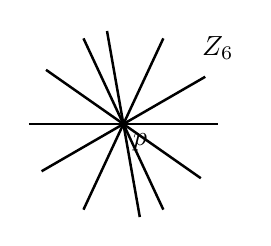
\begin{tikzpicture}[scale=0.4]
% Six lines passing through a common point p at the origin
% Draw the six lines without inline labels
\foreach \theta in {115,-80,65,-35,30,0} {
    \draw[rotate=\theta, line width=0.9pt] (-3,0) -- (3,0);
}
% Common intersection point p
\fill (0,0) circle (2pt) node[below right] {$p$};

% Optional label
\node at (3,2.4) {$Z_6$};
\end{tikzpicture}
    \caption{A 6-cross in $\mathbb{P}^3$.}
    \label{fig:Z_6}
    \end{figure}
    \begin{definition}
        An $m$-cross is a union of $m$ distinct lines $l_1, l_2, \dots, l_m$ in $\mathbb{P}^3$ which intersect at a common point $p$ and lying in a common plane $H$. We will write $Z_m = \bigcup_{i=1}^m l_i$.
    \end{definition}
\end{frame}

\begin{frame}
        \begin{theorem}
        Given an $m$-cross, we can find a smooth hypersurface of degree $d$ including it if and only if $d = 1$ or $d \geq m$.
    \end{theorem}

    Key idea: An automorphism of $\mathbb{P}^3$ can be used to move an $m$-cross into a position where we can explicitly construct such a surface. Explicitly, we move the lines to 
    \[l_1 = (\alpha : \beta : 0 : 0), \ l_2 = (\alpha : 0 : \gamma : 0), \ l_3=(\alpha: \lambda_3 \delta : \delta: 0), \dots, l_m = (\alpha :\lambda_m  \delta : \delta : 0)\]
\end{frame}

\begin{frame}
    \begin{itemize}
        \item If $d=1$, we can take $X = H$.
        \item If $1 < d < m$, no such surface exists. Consider a surface $X \subset \mathbb{P}^3$ of degree $d$ containing an $m$-cross $Z_m$, and a line in $H$ not passing through $p$. We use Bezout's theorem to see that this line must intersect $X$ in at least $d$ points, and since it intersects each line, we must have $d \geq m$ when $X$ is not equal to $H$.
        \item If $d \geq m$, we can construct such a surface. We consider a linear system with base locus $Z_m$, and find a surface which is smooth on $Z_m$. Then we apply Bertini's theorem to see that a general member of the linear system is smooth away from $Z_m$. Then we can find a surface of degree $m$ containing $Z_m$.
    \end{itemize}
\end{frame}

\begin{frame}
    \begin{theorem}
        Let $A_m = \{S_d \subseteq \mathbb{P}^3 \mid Z_m \subset S_d\} \subseteq \{S_d \subseteq \mathbb{P}^3\}$ be the set of degree $d$ surfaces containing a general $Z_m$. Then $\dim{A_m} = \binom{d-m+2}{2} + \binom{d+2}{3} - 1$.
    \end{theorem}
\end{frame}

\begin{frame}{$m$-gon}
    \begin{definition}
        An $m$-gon is a union of $m$ lines $l_1, l_2, \dots, l_m$ such that $l_i$ intersects $l_{i+1}$ for $1 \leq i < m$, and $l_m$ intersects $l_1$. We will write $C_m = \bigcup_{i=1}^m l_i$ and denote the intersection points as $p_i = l_i \cap l_{i+1}$ for $1 \leq i < m$, and $p_m = l_m \cap l_1$.
    \end{definition}
    Regularity.
    \begin{theorem}
        Given a regular $m$-gon, we can find a smooth surface $S_d$ of degree $d$ including it when $m < \binom{d+3}{3}\cdot \frac{1}{d}$.
    \end{theorem}
    % \begin{figure}
    %     \centering
    %     % define a macro that draws a m-gon placed on a circle
\newcommand{\mgon}[1]{%
    \begin{tikzpicture}[scale=1, every node/.style={font=\small}]
        % radius of circle
        \def\R{2.2cm}
        \pgfmathparse{int(#1)}\let\K\pgfmathresult
        % place the points on a circle and draw the lines
        \foreach \i in {1,...,\K} {
            \pgfmathsetmacro{\ang}{90 - 360*(\i-1)/\K}
            \coordinate (P\i) at (\ang:\R);
        }
        % draw the edges (lines) and label them l_i at the midpoint
        \foreach \i in {1,...,\K} {
            \pgfmathtruncatemacro{\j}{ifthenelse(\i==\K,1,\i+1)}
            \draw[line width=0.9pt] (P\i) -- (P\j) node[midway, above, font=\small] {$l_{\i}$};
        }
        % draw and label intersection points p_i (small filled dots)
        \foreach \i in {1,...,\K} {
            \fill (P\i) circle (2.4pt) node[below right=1mm and 1mm] {$p_{\i}$};
        }
    \end{tikzpicture}
}

% Example: draw a 7-gon (change the number to any m you want)
\mgon{7}
    %     \caption{7-gon drawn in a plane.}
    %     \label{fig:m-gon}
    % \end{figure}
\end{frame}

\begin{frame}[fragile]
    Observe this with the sequence:
    \[0 \to \mathcal{I}_{C_m}(d) \to \mathcal{O}_{\mathbb{P}^3}(d) \to \mathcal{O}_{C_m}(d) \to 0.\]
    Taking cohomology gives the long exact sequence:
    \[
        \begin{tikzcd}[sep=small]
        0 \ar[r]
        & H^0(\mathcal{I}_{C_m}(d)) \ar[r]
        & H^0(\mathcal{O}_{\mathbb{P}^3}(d)) \ar[r]
        & H^0(\mathcal{O}_{C_m}(d)) \ar[controls={+(3,-1.5) and +(-3,1.5)}]{dll} \\
        {}
        & H^1(\mathcal{I}_{C_m}(d)) \ar[r]
        & H^1(\mathcal{O}_{\mathbb{P}^3}(d)) \ar[r]
        & H^1(\mathcal{O}_{C_m}(d)) \ar[controls={+(3,-1.5) and +(-3,1.5)}]{dll} \\
        {}
        & H^2(\mathcal{I}_{C_m}(d)) \ar[r]
        & H^2(\mathcal{O}_{\mathbb{P}^3}(d)) \ar[r]
        & \dots
        \end{tikzcd}
    \]
\end{frame}

\begin{frame}[fragile]
    Note that 
    \[
        \begin{tikzcd}[sep=small]
        0 \ar[r]
        & H^0(\mathcal{I}_{C_m}(d)) \ar[r]
        & H^0(\mathcal{O}_{\mathbb{P}^3}(d)) \ar[r]
        & H^0(\mathcal{O}_{C_m}(d)) \ar[controls={+(3,-1.5) and +(-3,1.5)}]{dll} \\
        {}
        & H^1(\mathcal{I}_{C_m}(d)) \ar[r]
        & \alert<1>{H^1(\mathcal{O}_{\mathbb{P}^3}(d))} \ar[r]
        & H^1(\mathcal{O}_{C_m}(d)) \ar[controls={+(3,-1.5) and +(-3,1.5)}]{dll} \\
        {}
        & H^2(\mathcal{I}_{C_m}(d)) \ar[r]
        & \alert<1>{H^2(\mathcal{O}_{\mathbb{P}^3}(d))} \ar[r]
        & \dots
        \end{tikzcd}
    \]
\end{frame}

\begin{frame}[fragile]
    \begin{example}
        Cohomology of a 4-gon.
    \end{example}
\end{frame}

\begin{frame}{$m$-chain}
    \begin{definition}
        An $m$-chain is a union of $m$ lines $l_1, l_2, \dots, l_m$ such that $l_i$ intersects $l_{i+1}$ for $1 \leq i < m$. We will write $Q_m = \bigcup_{i=1}^m l_i$ and denote the intersection points as $p_i = l_i \cap l_{i+1}$ for $1 \leq i < m$. 
    \end{definition}
    Regularity.
    \begin{theorem}
        A regular 6-chain is included in a unique cubic surface, which is singular.
    \end{theorem}
\end{frame}

\begin{frame}{4-chain}
    4-chains.
\end{frame}

\begin{frame}{6-chain}
    6-chains.
\end{frame}

\begin{frame}{Computational results}
    Computations.
\end{frame}

\end{document}